% QM/MM
% Documentation copied from https://www.ks.uiuc.edu/Research/qmmm/.

\section{Hybrid QM/MM Simulations}
\label{section:qmmm}

% This brief introduction aims at providing some basic context 
% to the following description of capabilities and commands 
% available in NAMD's QM/MM interface.

Even though molecular mechanics (MM) force-fields are based on
quantum mechanical calculations and experimental observations,
only quantum mechanics (QM) can give a complete and accurate
understanding of many biochemical processes, particularly those
involving chemical reactions or charge redistribution.
Nevertheless, even with the advanced hardware technology available today,
the computational cost of studying nanosecond-long dynamics of entire
systems relying solely on QM methodologies is usually prohibitive.
A common route to circumvent this cost barrier is to confine the
QM formalism to a sub-region of a system and to include the effects
of the surrounding system through MM simulations,
leading to hybrid QM/MM simulations~\cite{SENN2009}.

NAMD's comprehensive QM/MM suite~\cite{MELO2018} was developed to provide
easy setup, visualization and analysis of QM/MM simulations through
the graphical user interface VMD/QwikMD~\cite{RIBE2016},
and a broad range of QM methods through NAMD's new ``QMForces" module.
The QM/MM interface in NAMD supports the simulation of many
independent QM regions, and smooth integration with a vast collection
of enhanced sampling methods. In hybrid QM/MM simulations,
NAMD offloads part of its standard force and energy calculations
to a QM program, either through native interfaces to
MOPAC~\cite{STEW90,MAIA2012} or ORCA~\cite{NEES2012},
or through a flexible generic interface requiring a wrapper script,
where exemplary Python wrappers are provided for Gaussian,
TeraChem and Q-CHEM.
Multiple QM-MM coupling schemes are implemented, allowing for both
mechanically and electrostatically embedded QM regions to be used
(see description in Nature Methods~\cite{MELO2018}).
QM/MM simulations require the same input files used for classical MD,
with additional options in the configuration file.
QM and MM atoms covalently bound are usually treated by redistributing
the MM atom's charge over its nearest MM neighbors and by capping
the QM atom with a hydrogen atom,
as shown in Figure~\ref{fig:hybrid_qmmm} for a solvated
tri-alanine QM/MM calculation using the NAMD/ORCA interface.
Tests of the QM/MM interface for accuracy, stability and performance,
are provided as supporting information in Nature Methods~\cite{MELO2018}. 

If employing NAMD QM/MM please cite:
\begin{quote}
NAMD goes quantum: An integrative suite for hybrid simulations.
Melo*, M. C. R.; Bernardi*, R. C.; Rudack T.; Scheurer, M.; Riplinger, C.;
Phillips, J. C.; Maia, J. D. C.; Rocha, G. D.; Ribeiro, J. V.;
Stone, J. E.; Neese, F.; Schulten, K.; Luthey-Schulten, Z.;
Nature Methods, 2018 (doi:10.1038/nmeth.4638)
\end{quote}

\begin{figure}[tbp]
\centering
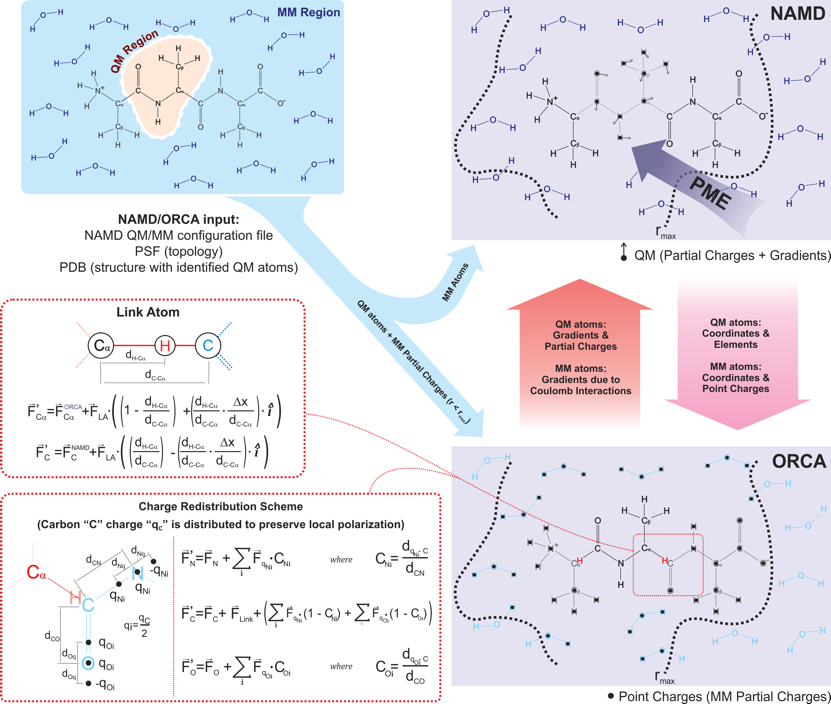
\includegraphics[width=6in]{figures/hybrid_qmmm_diagram.png}
\caption[Hybrid QM/MM NAMD]{%
Graphical representation of NAMD-ORCA interconnection.
Only the contribution of MM charges beyond rmax are
calculated by NAMD (via PME), with the direct electrostatic
calculation performed by ORCA.
The image assumes the charge shift redistribution scheme,
where the partial charge of the linking MM atom is shifted
to its nearest MM neighbors.
}
\label{fig:hybrid_qmmm}
\end{figure}


\subsection{Division of Labor}

The basic idea behind a hybrid QM/MM simulation in NAMD is to use 
a classical force field to treat the classical atoms in the system 
(or ``MM atoms"), and pass the information that describes the quantum 
atoms in the system (or ``QM atoms") to a Quantum Chemistry (QC) software, 
which is expected to produce gradients for all QM atoms, as well as 
the total energy of the QM region (and optionally partial charges). 
All bonded and non-bonded interactions among MM atoms are handled 
by NAMD's force field. Similarly, all bonded and non-bonded interactions 
among QM atoms are handled by the QC software in its chosen theory level. 
Treatment of covalent bonds between QM and MM atoms will be described 
in a following section.

The non-bonded interactions between QM and MM atoms are handled differently, 
and can be modified and regulated by the user. 
Van der Waals interactions are always calculated, and can be done 
using either the default force field parameters, or specific 
(user-defined) parameters for QM atoms. 
Parameter modifications for QM atoms have been proposed 
in order to compensate for over-polarization that these atoms 
may exhibit in hybrid QM/MM simulations. 
Larger van der Waals radii and/or shallower well depths 
should then be provided for all element types that occur 
among QM atoms (see the ``qmVdwParams" keyword).


\subsection{Mechanical and Electrostatic Embedding}

Electrostatic interactions between QM and MM atoms deserve 
a more detailed discussion due to the abundance and diversity 
of available alternatives. 
The first decision to be made is whether there will be electrostatic 
interactions between the two portions of a system, QM and MM. 
In the ``mechanical embedding" scheme, only positions and elements 
of atoms in the QM region are passed on to the chosen QC software 
for energy and force calculations. 
This way, QM and MM atoms share only van der  Waals interactions.

% Figure 1 for QM/MM
\begin{figure}[tbp]
\centering
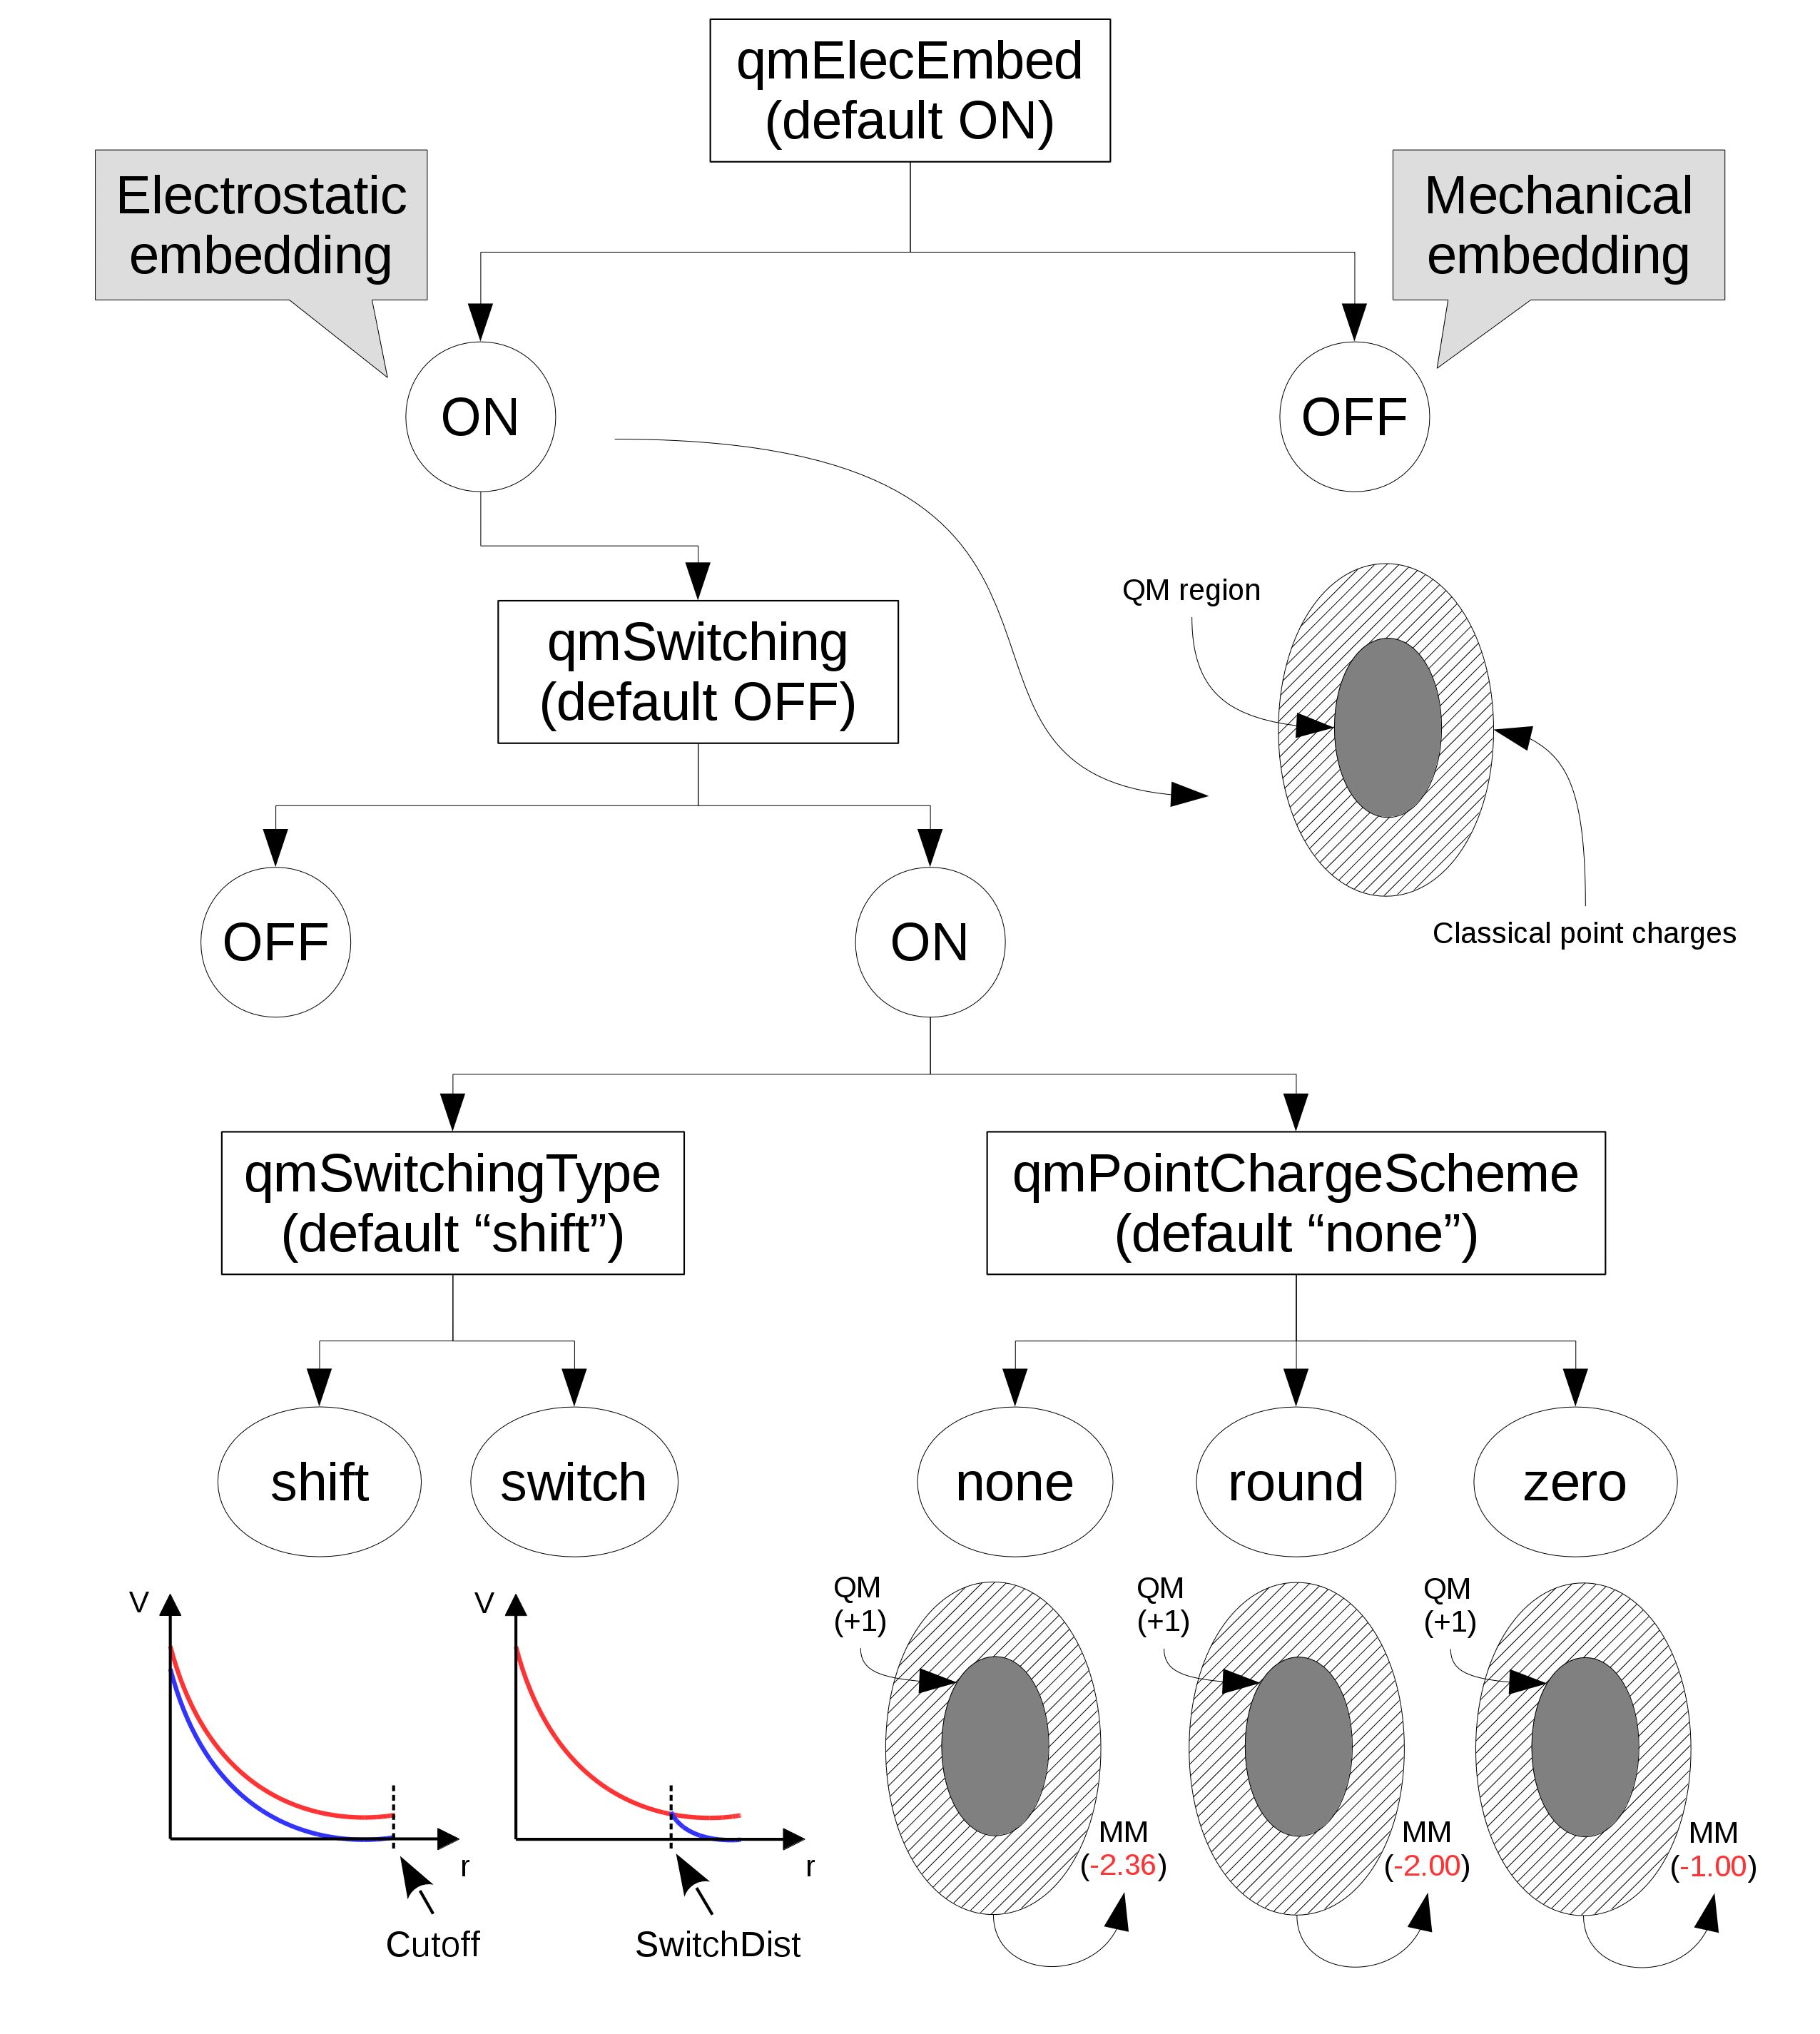
\includegraphics[width=5in]{figures/OptionsDiagram.png}
\caption[Diagram of classical point charge options.]{%
Diagram of options that control the use and manipulation of 
classical point charges. Default values are indicated below their 
respective keyword. ``Cutoff" and ``SwitchDist" are keywords used in 
NAMD to configure the calculations of electrostatic and van der Waals 
interactions. 
}
\label{fig:qmmm_options}
\end{figure}

In the ``electrostatic embedding" scheme, on the other hand, 
the partial charges of MM atoms surrounding all QM atoms 
are used to approximate the electrostatic environment where QM atoms 
are found (the scheme is selected with the ``qmElecEmbed" keyword). 
See Figure~\ref{fig:qmmm_options}.
This process can be customized in a variety 
of ways, the first of which is deciding if a smoothing function will 
be used to avoid an abrupt decay in electrostatic force 
due to the cutoff used in the selection of surrounding point charges
(this option is activated with the ``qmSwitching" keyword).

Classical point charge utilization can be further customized 
by choosing which smoothing function will be used, 
and if the total charge of selected partial charges should be 
modified to (A) have a whole charge or (B) have a complementary 
charge to that of the QM region, so that the sum of charges 
from QM atoms and classical partial charges add to zero
(see Figure~\ref{fig:qmmm_options}).

With electrostatic embedding, QM atoms are influenced by the charges 
in the classical region. In order to balance the forces acting on the 
system, NAMD uses partial charges for the QM atoms to calculate 
the electrostatic interaction with classical point charges. 
There are two possibilities for the origin of the QM partial charges: 
the original partial charges found in the force field parameter files 
can be used, or updated partial charges can be gathered at each step 
from the QC software output 
(controllable through the ``qmChargeMode" keyword). 
The continuous update in charge distribution allows for a partial 
re-parameterization of the targeted molecule at each time step, 
which can lead to an improved description of the interactions 
of a ligand as it repositions over the surface of a protein, 
for example, or as it moves through a membrane.

In case PME is activated by the user, NAMD will automatically apply 
the necessary corrections to handle the QM region, allowing it to be 
influenced by long range interactions from the entire system.


\subsection{Covalent Bonds Divided by the QM/MM Barrier}

Hybrid QM/MM simulations of biomolecular systems often present 
situations where only a portion of a molecule should be treated 
quantum mechanically, usually to save computational resources 
since the cost of simulating QM regions rises rapidly with the 
number of simulated toms. In order to deal with chemical bonds 
that are split by the QM/MM division of the biomolecular system, 
that is, bonds that have one atom in the quantum (QM) region and 
another in the classical (MM) region (we will call these ``QM/MM bonds"), 
NAMD makes approximations to the molecular system in order to bridge 
differences in simulation type (QM vs.\ MM), and minimize errors involved 
in the QM/MM division of the system
(Figure~\ref{fig:qmmm_bond_treatment} A and B).

\begin{figure}[tbp]
\centering
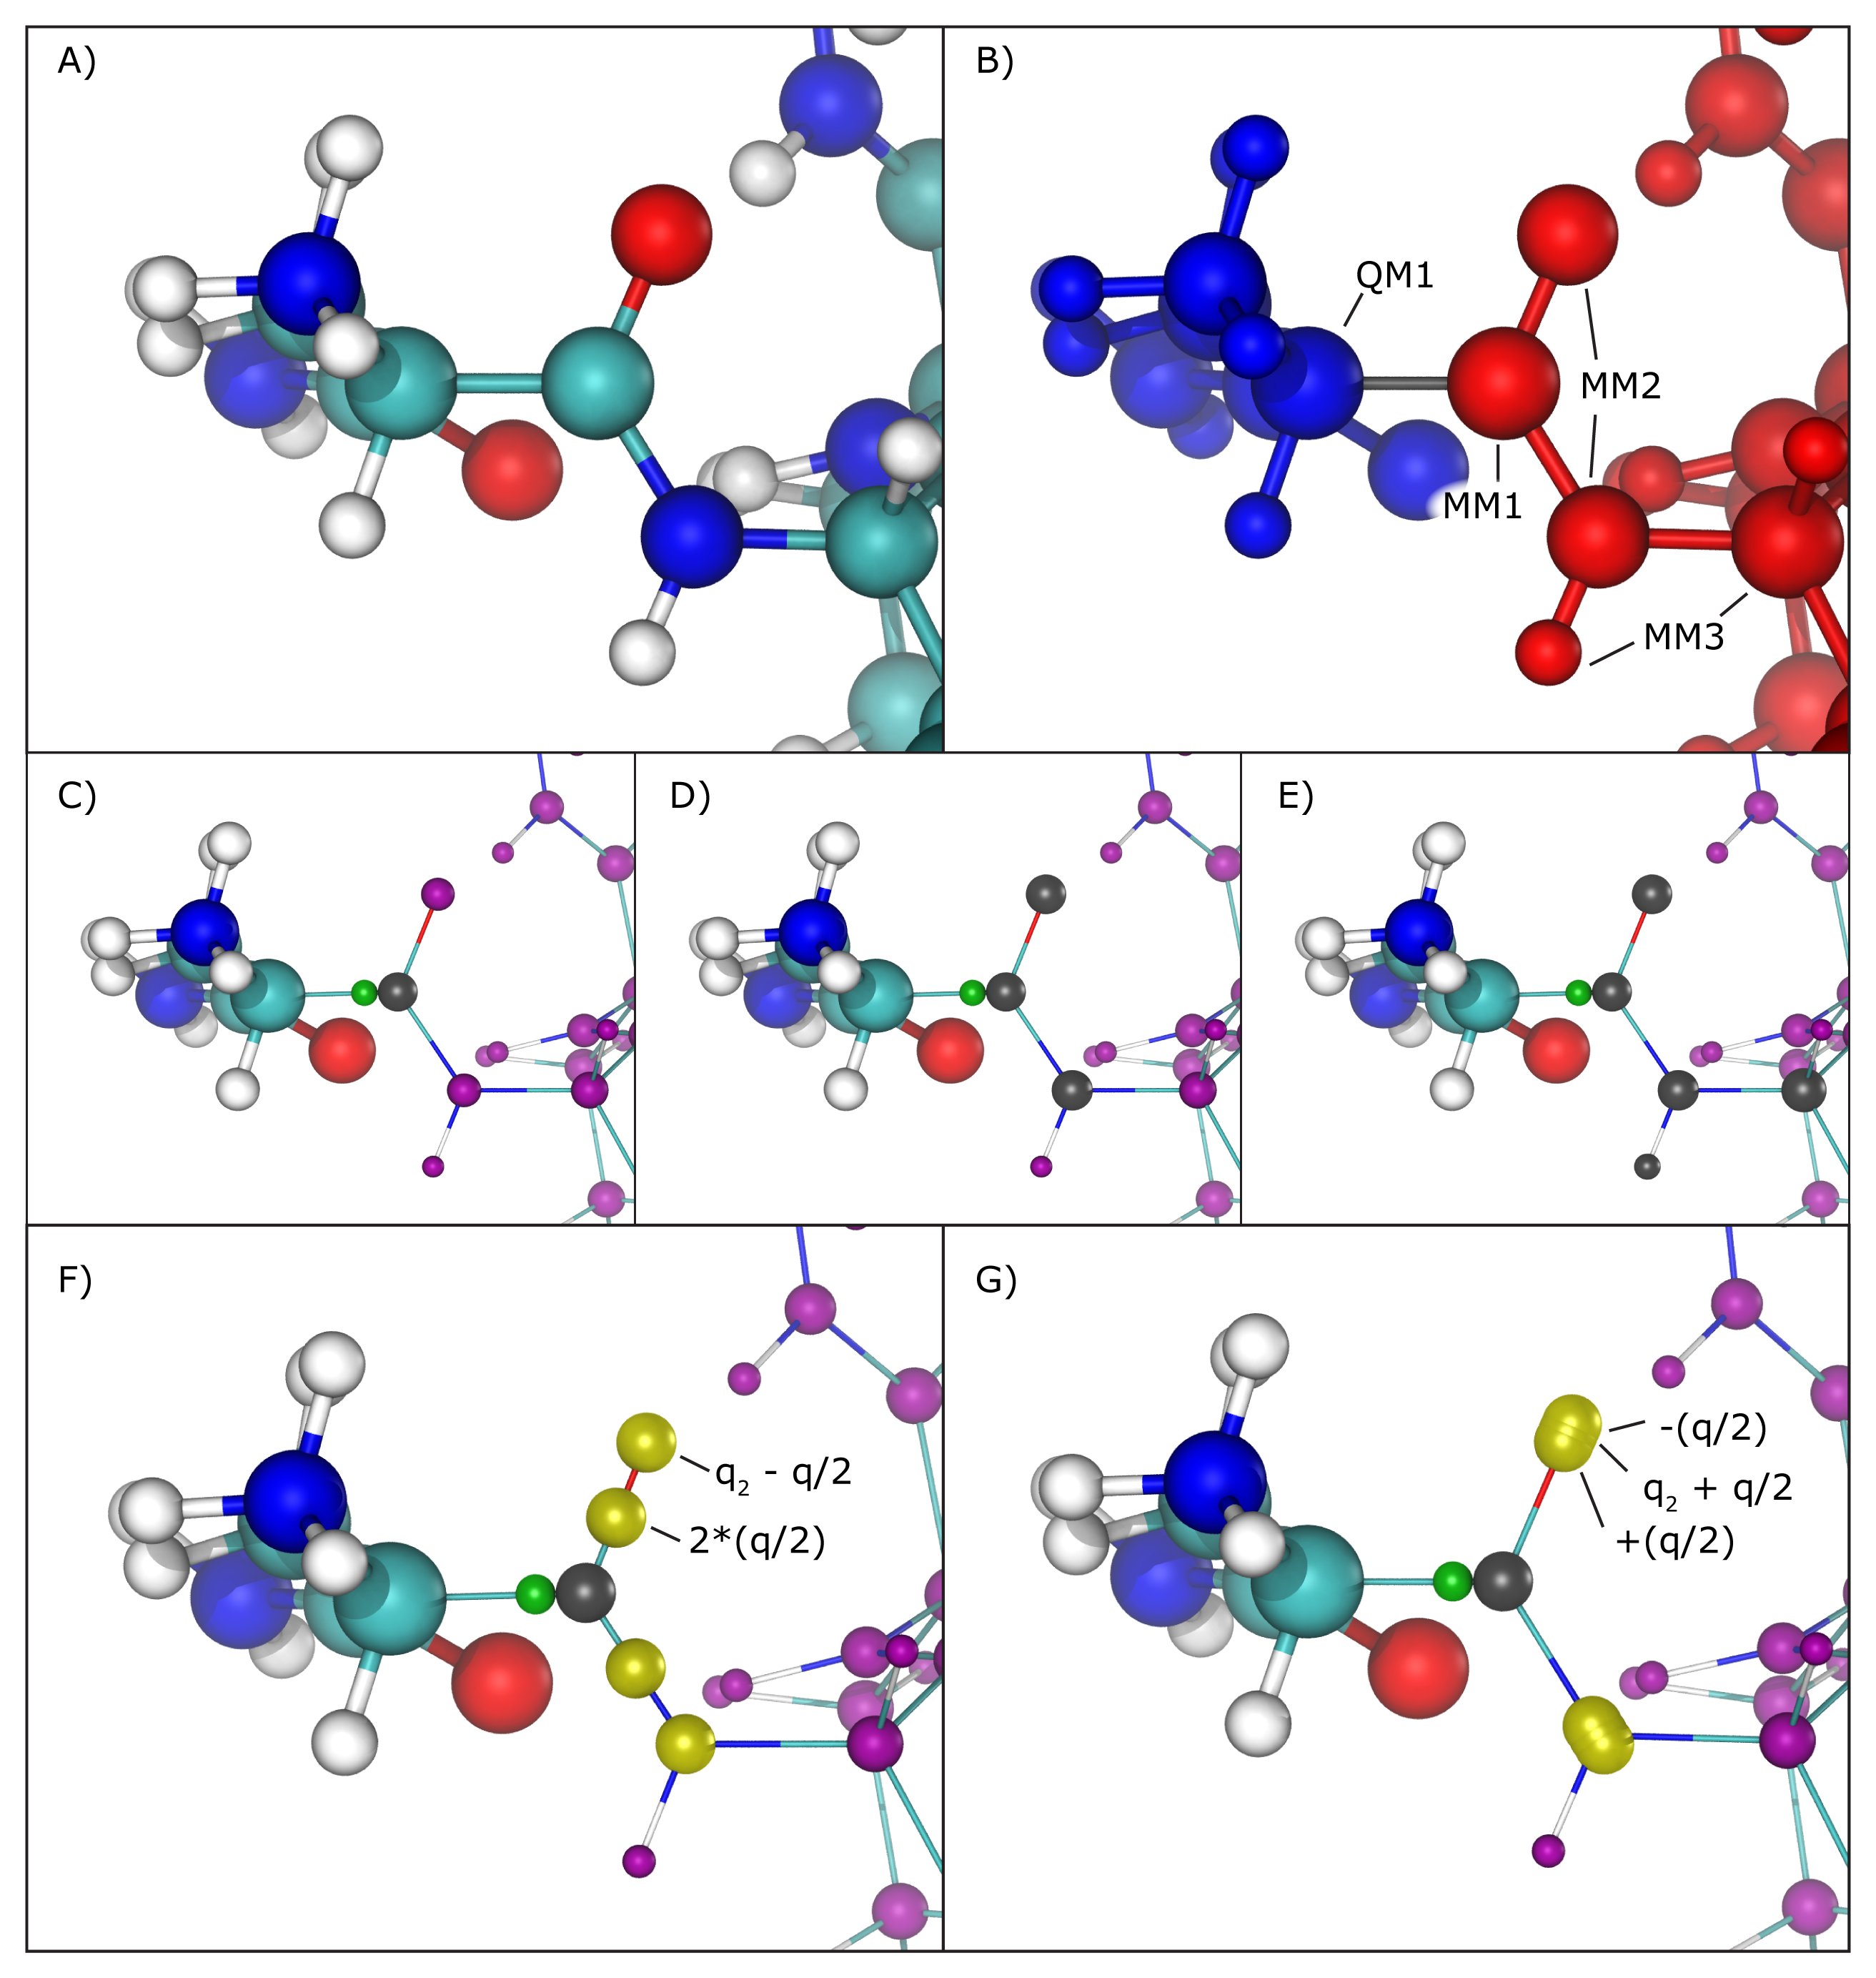
\includegraphics[width=5in]{figures/QMMMBond_2bonds-01.png}
\caption[Treatment of QM/MM bonds]{%
Treatment of QM/MM bonds.
A) Illustration of all atoms in the vicinity of the QM/MM bond, 
colored by element: cyan for carbon, white for hydrogen, 
blue for nitrogen and red for oxygen. 
B) To the left, in blue, is the region that will be treated with 
the chosen QC software. To the right, in red, the region treated 
classically by NAMD. The bond in gray is the one crossing the 
QM/MM division. The atom marked as \textbf{QM1} is the quantum atom 
directly connected to the classical atom on the other side of the 
QM/MM division. Analogously, the atom marked as \textbf{MM1} is the 
classical atom directly connected to the quantum atom on the other 
side of the QM/MM division. Atoms marked as \textbf{MM2} are directly 
bonded to the \textbf{MM1} atom, and atoms marked \textbf{MM3} are 
directly bonded to \textbf{MM2} atoms. 
C) \textbf{Z1} method. Ignored partial charges are indicated in the image 
with a gray sphere taking the place of its respective classical atom. 
Directly adjacent to MM1 is a green sphere representing the link atom 
that is placed along the QM1-MM1 covalent bond. All remaining partial 
charges representing classical atoms that are passed on to the QC software
are indicated in purple spheres. 
D) \textbf{Z2} method.  
E) \textbf{Z3} method. 
F) RCD method. Virtual point charges, are represented in yellow spheres. 
The text indicates the total charge placed at each position, 
where \textbf{q} indicates the charge of the MM1 atom and \textbf{q2} 
represents the partial charge of the MM2 atom at that position. 
The yellow spheres at MM2 atom positions indicate their partial charge 
has been changed from its original value. 
G) CS method. Since in this case the virtual point charges are placed 
very close to the MM2 atom position, the yellow spheres representing 
them show significant overlapping.
}
\label{fig:qmmm_bond_treatment}
\end{figure}


\subsubsection{Link Atoms}

As previously mentioned, the information regarding atoms in the QM region 
is passed on to the chosen QC software, that is, their respective 
positions and element types, but in order to maintain (or approximate) 
the effect of the chemical bond between the QM atom and the MM atom, 
NAMD creates and places a link atom (usually a hydrogen) along the 
``broken" QM/MM bond. The user can fine-tune this process by choosing 
the method of placement of the link atom and even the element of 
such atom (keywords ``qmBondDist" and ``qmLinkElement").

The introduction of the link atom will invariably place it very near 
the classical atom involved in the QM/MM bond, therefore the use 
and placement of partial charges from classical atoms becomes
highly relevant. Under the mechanical embedding scheme, the QC software 
only receives the atoms in the QM region and the link atoms created
to approximate QM/MM bonds, so no manipulation of partial charges is 
required. On the other hand, usual QM/MM simulations are done under 
the electrostatic embedding scheme, in which case the partial charges
of classical atoms involved in the QM/MM bonds and classical atoms 
directly connected to them require special treatment.


\subsubsection{Point Charge Alterations}

Several methods have been proposed to handle this situation, and the 
QM/MM interface developed here implements the most widely accepted ones.
One can be chosen using the ``qmBondScheme" keyword
(Figure~\ref{fig:qmmm_bond_treatment} C to G). 
In all implemented methods, the classical atom participating in the 
QM/MM bond (MM1 atom) does not have its partial charge passed on 
to the QC software, since this would create excessive repulsion 
(or attraction) on the link atom. This is, in fact, the entirety of 
the ``Z1" method: ignoring the partial charge of the MM1 atom. 
Analogously, ``Z2" and ``Z3" ignore all partial charges up to 
MM2 and MM3 atoms, respectively
(Figure~\ref{fig:qmmm_bond_treatment} C to E).

The Redistributed Charge and Dipole (RCD) method
(Figure~\ref{fig:qmmm_bond_treatment} F)
is more elaborate, as it rearranges the partial charge of the 
MM1 atom (indicated as $q$) so that the total charge of the region 
is maintained as well as the dipole moments of the bonds between 
MM1 and MM2 atoms. This is done by creating ``virtual" point charges, 
which are passed on to the QC software as if they represented 
partial charges of classical atoms. More specifically, the RCD method 
creates a virtual point charge in the middle of all MM1-MM2 bonds 
with a charge of $2q/n$, where $n$ is the number of 
MM2 atoms connected to MM1, and also subtracts a charge $q/n$ 
from each of the MM2 atoms, so that the total charge of the region 
remains constant while approximating the dipole moment of the 
MM1-MM2 bonds. This way there will be no point charge placed at the 
position of the MM1 atom, but its partial charge is not simply removed, 
it is redistributed.

A similar approach is taken by the Charge Shifting (CS) method 
(Figure~\ref{fig:qmmm_bond_treatment} G).
In this case, the MM1 partial charge is equally 
distributed across the MM2 atoms, and two virtual point charges 
are placed along the direction of the MM1-MM2 bond, one before 
the MM2 atom and one after, each one with a charge of $+q/n$ 
and $-q/n$ respectively. This method will also keep the 
total charge of the region constant while trying to preserve 
the local dipoles formed by all MM1-MM2 bonds.


\subsubsection{Link Atom Charge and Charge Groups}

Along with the gradient over all QM atoms, NAMD can also use 
the partial charge derived from the QC calculation to update 
the charge distribution of atoms in the QM region. 
When a QM/MM bond exists, however, part of the charge of the 
region will be placed on the link atom, and in order to keep the 
charge of the QM region constant, the link atom charge is 
re-distributed on the QM region. This seemingly simple mechanism 
can cause problems unless special care is be taken when deciding 
which bond will mark the division of QM and MM regions.

Many force fields divide the topologies of biomolecules in 
``charge groups"
(Figure~\ref{fig:qmmm_chargegroups} A and B).
What this means is that 
not only will the partial charges of all atoms of a molecule 
add up to the whole number that represents the charge of the molecule, 
they will also add up to whole numbers in sub groups of atoms 
(look for the ``GROUP" statements in
\url{http://www.ks.uiuc.edu/Training/Tutorials/namd/namd-tutorial-unix-html/node24.html}
to see an example). 
Therefore, one needs to make sure that the chosen QM/MM bond(s) sits
in between ``charge groups", so the total sum of partial charges 
of atoms defining a QM region is a whole number. This is especially 
important in order to keep the total charge of the system constant. 
Since the QC calculation will always distribute a whole charge over 
all atoms of a system (QM atoms plus a link atom), if the partial charge 
of QM atoms is not initially a whole number, it will be forced into 
a whole number after the first QC step, where the charge of the link atom 
is distributed over the QM region. This will create a mismatch between 
QM and MM charges, changing the total charge of the entire system 
(QM plus MM regions).

\begin{figure}[tbp]
\centering
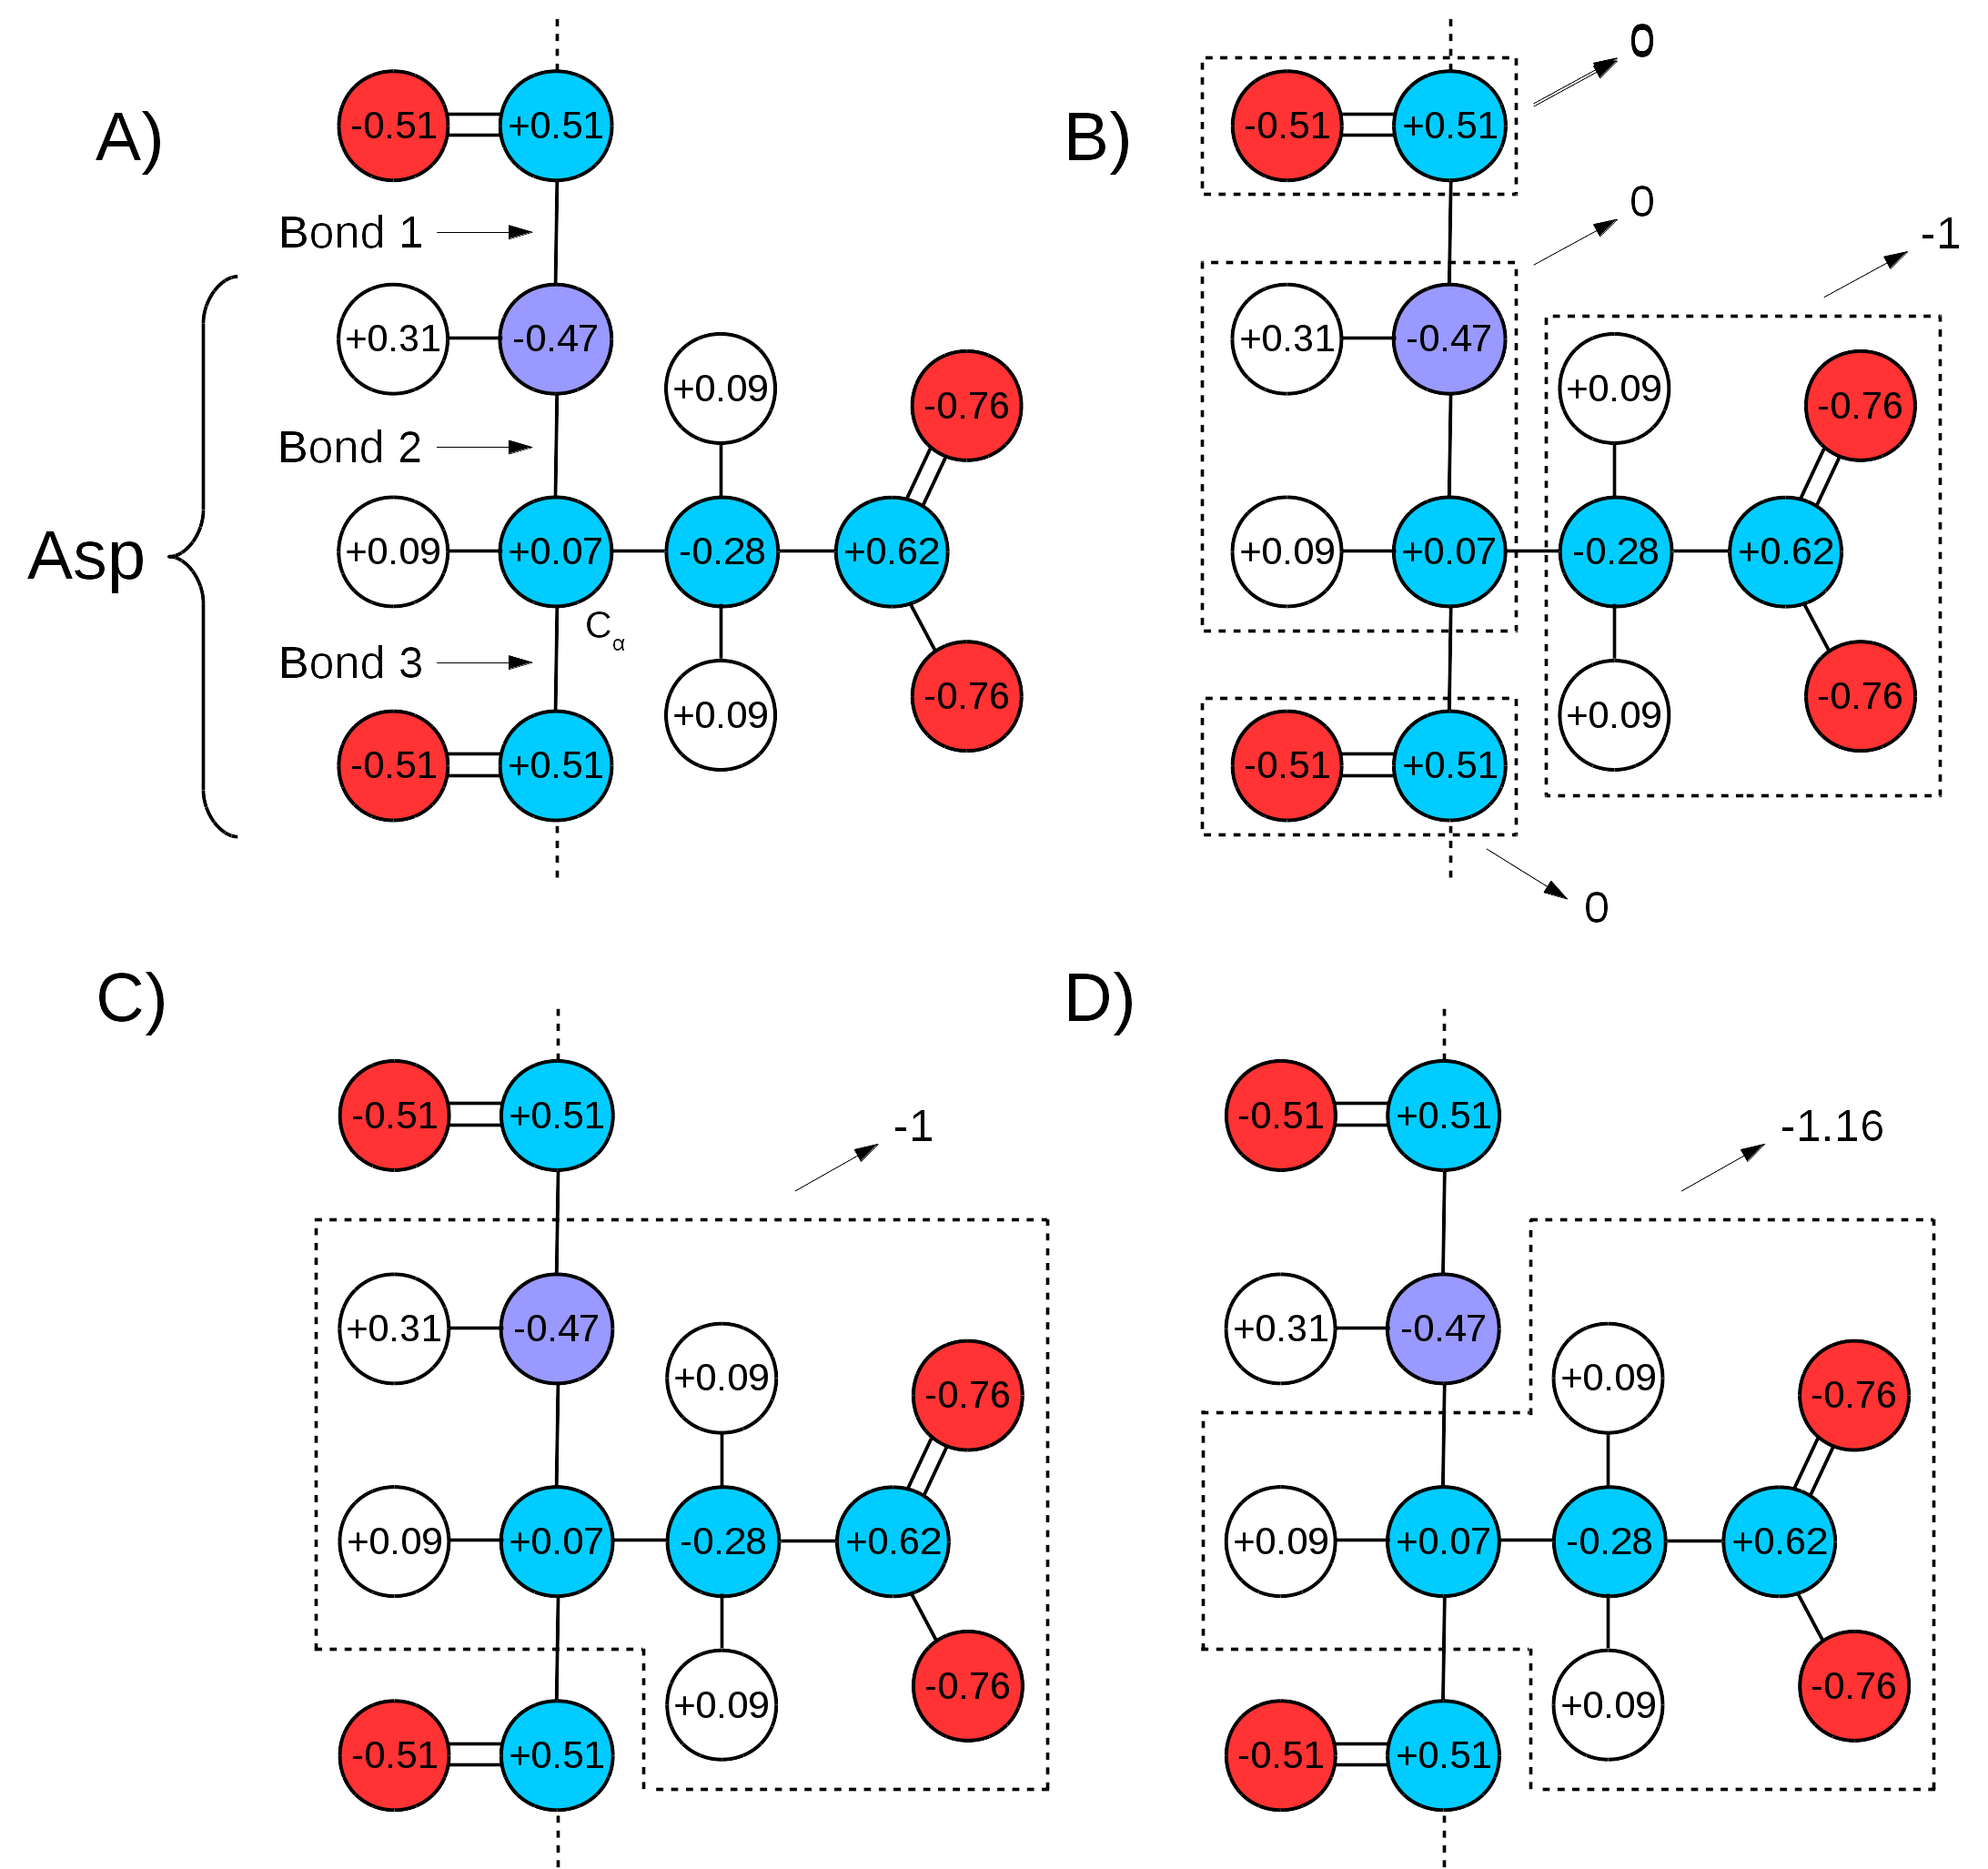
\includegraphics[width=5in]{figures/ChargeGroupDiagram.png}
\caption[Charge Groups and QM/MM Bonds]{%
Charge Groups and QM/MM Bonds.
A) Illustration of aspartate and the distribution of charge over its 
atoms as in CHARMM36 force field parameters. Circles in red indicate 
oxygen atoms, blue indicate nitrogen atoms, cyan for carbon atoms, 
and white for hydrogen atoms. ``Bond 1" indicates the peptide bond,
``Bond 2" indicates the one between the alpha carbon and the peptide bond 
nitrogen, and ``Bond 3" the bond between the alpha carbon and the peptide 
bond carbon. 
B) Charge groups are indicated with dashed squares, 
along with their total charges. 
C) Depiction of the atoms in the QM region if Bonds 1 and 3 are used to 
separate it from the MM region. The total charge of QM region is $-1$. 
D) Depiction of QM region if the same is defined by Bonds 2 and 3. 
In this case, the total charge of QM region is $-1.16$.
}
\label{fig:qmmm_chargegroups}
\end{figure}

An example can be seen in Figure~\ref{fig:qmmm_chargegroups},
bonds 1 and 3 are chosen as the QM/MM bonds,
the charge distribution seen in Figure~\ref{fig:qmmm_chargegroups} C shows 
a whole charge for the QM region (and consequently for the MM region). 
Therefore, any charge placed on link atoms can be redistributed 
to the QM atoms with no change in total system charge. However, 
if bonds 2 and 3 are chosen for the QM/MM bond
(Figure~\ref{fig:qmmm_chargegroups} D), 
the charge of the MM region would be $+1.16$, while the charge 
of the QM region would be $-1.16$. Since the QC calculation would 
place a pre-determined whole charge on the region ($-1$, in this case), 
the updated charge of the QM region after the first simulation step 
would change the total charge of the system to $+0.16$, in this example.


\subsection{Custom Quantum Chemistry Software}

In order to offer the broad range of tools and technologies present 
in NAMD to all researchers who develop and/or employ specialized 
Quantum Chemistry tools, the QM/MM interface is prepared to utilize 
any QC tool that can be wrapped in a script that converts input and 
output files to specified formats. This flexible interface will 
improve development and testing of new tools, as well as their 
quick integration utilization in hybrid dynamics.

We currently provide 
in the \texttt{libs/qmmm/} directory
(and mirrored at
\url{http://www.ks.uiuc.edu/Research/qmmm/Scripts/})
Python wrapper scripts for GAUSSIAN, TeraChem, and Q-Chem.
Other wrapper scripts can be generated, based on these templates,
in any other language,
as long as they are provided to NAMD in an executable form.
Although natively supported,
we also provide a python wrapper script for ORCA,
with extended comments explaining the format in which NAMD will write 
data for the QC software and the format in which NAMD expects to find 
the results.


\subsection{Independent QM Regions}

Aiming at large macromolecular simulations that could take advantage 
of localized QM resolution, NAMD allows the user to set up multiple 
independent QM regions in the same molecular system. For example, 
one could study a multimeric complex that contains several active sites 
and have all active sites be calculated with a chosen QC software 
simultaneously (Figure~\ref{fig:qmmm_multiple_grid}).
Each active site would be calculated 
independently of all others, by its own execution of the QC software, 
keeping the calculation cost low and without impacting the overall 
efficiency of the simulation, since all QM regions would be calculated 
in parallel.

\begin{figure}[tbp]
\centering
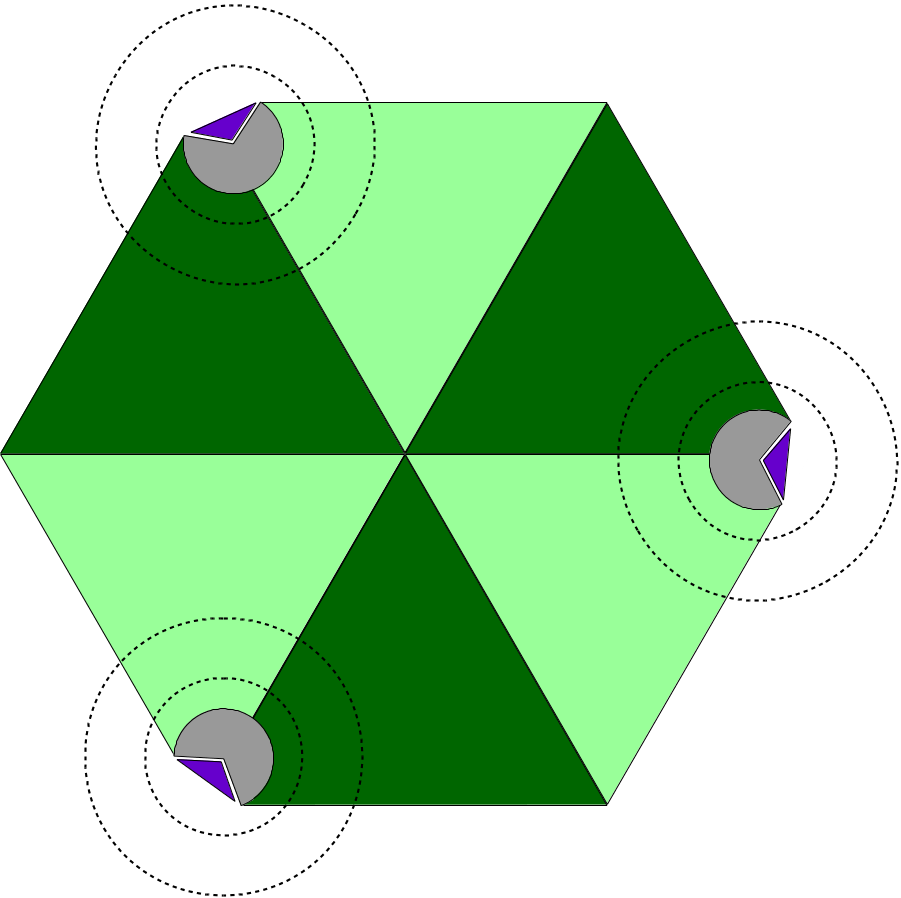
\includegraphics[width=5in]{figures/MultipleQMDiagram.png}
\caption[Diagram of Multiple Grid Regions]{%
Diagram of Multiple QM Regions. 
The illustration depicts a hetero-hexameric complex 
(light and dark green triangles) that combine to create three active sites 
(in gray). Active sites are bound to a target molecule (purple triangle). 
The inner and outer dashed circles represent, respectively, the boundary 
of a QM region and the limits of the classical point charge shell around 
that region.
}
\label{fig:qmmm_multiple_grid}
\end{figure}

Identifying the different QM regions and which atoms belong to each 
one of them can be simply accomplished in the input PDB file, 
or in a dedicated PDB file (keyword ``qmParamPDB"). Since each region 
can contain different sets of molecules, their charges and multiplicities 
are indicated separately (see keywords ``qmCharge" and ``qmMult").

For simulations of large systems that are distributed across several 
computer nodes, one can control how many independent QM regions are 
calculated in each node. This would prevent large simulations from 
running out of memory if two or more large QM regions are placed 
in the same node (see keyword ``qmSimsPerNode").


\subsection{Keywords}

\begin{itemize}
\setlength{\itemsep}{0.4cm}

\item
\NAMDCONFWDEF{qmForces}{Calculate QM?}{yes or no}{no}{%
Turns on or off the QM calculations.
}

\item
\NAMDCONF{qmParamPDB}{Set QM atoms}{PDB file}{%
Name of an optional secondary PDB file where the OCCupancy
or BETA column has the indications for QM or MM atoms.
QM atoms should have an integer bigger than zero (0) and 
MM atoms should have zero as the beta or occupancy field. 
The same file may have indications for bonds between a QM atom 
and an MM atom. This should be provided in case the PDB file 
passed to the ``coordinates" keyword already has data on its 
beta or occupancy columns, such as when a SMD simulations 
is being performed.
}

\item
\NAMDCONF{qmColumn}{Which column?}{``beta" or ``occ"}{%
Indicates which column has the QM/MM field.
Required.
}

\item
\NAMDCONFWDEF{qmSimsPerNode}{Sims per node}{postive integer}{1}{%
Number of independent simultaneous QM simulations per node.
}

\item
\NAMDCONF{qmBondColumn}{Which bond column?}{``beta" or ``occ"}{%
Indicates which column has the QM/MM bond information.
This will tell NAMD which atoms are at the ends of a covalent bond
split by the QM/MM barrier, with one atom being quantum and
one being classical.
There is no default value.
If this parameter is provided,
NAMD will parse options for dealing with QM/MM bonds.
}

\item
\NAMDCONFWDEF{qmBondDist}{Use qmBondColumn value for distance?}%
{``on'' or ``off''}{off}{%
Indicates whether the value in the BondColumn will be used to define 
the distance between the QM atom and the Link Atom that will replace 
the MM atom in the QM system.
}

\item
\NAMDCONFWDEF{qmBondValueType}{Does qmBondColumn value give length or ratio?}%
{``len'' or ``ratio''}{len}{%
Indicates if the values in the BondColumn represent either 
the length (``len'') between the QM and link atoms or 
the ratio (``ratio'') between the QM-MM distance and 
the one which will be used as the QM-Link distance.
}

\item
\NAMDCONFWDEF{qmLinkElement}{Set link atom element}%
{string, for example ``4 9 Cl"}{H}{%
User defined link atom element. Two syntaxes are allowed:
if there is only one QM-MM bond, a string with the element symbol 
is allowed (such as ``H" or ``Cl"). If there are two or more bonds, 
the string needs to have the two atoms that compose the bond, 
and then the element (such as ``4 9 Cl"). 
The default element for all link atoms is hydrogen.
}

\item
\NAMDCONFWDEF{qmBondScheme}{Select QM-MM bond scheme}%
{``CS" or ``RCD" or ``Z1" or ``Z2" or ``Z3"}{CS}{%
Indicates what will be the treatment given to QM-MM bonds in terms 
of charge distribution and link atom creation and placement. 
CS: Charge Shift Scheme; RCD: Redistributed Charge and Dipole method; 
Z1: Only ignored MM1 partial charge, with no charge redistribution; 
Z2: Ignores MM1 and all MM2 partial charges, with no charge redistribution; 
Z3: Ignores MM1 and all MM2 and MM3 partial charges, 
with no charge redistribution.
}

\item
\NAMDCONFWDEF{qmBondGuess}{Guess QM-MM bonds from topology and QM atom definitions}%
{yes or no}{no}{%
With this option, NAMD will ONLY use QM region definitions and topology data to
determine QM-MM bonds. NAMD will ignore the user-provided QM bond column values
(in case the user assigned a value to the qmBondColumn variable and populated 
the column in the PDB file).
}

\item
\NAMDCONFWDEF{qmElecEmbed}{Should point charges be used in QM?}%
{``on" or ``off"}{on}{%
Indicates if classical point charges should be used in QM calculations.
}

\item
\NAMDCONFWDEF{qmSwitching}{Use switching on point charges?}%
{``on" or ``off"}{off}{%
This will scale down the point charges representing the classical 
system as to replicate the switching procedure that NAMD applies 
to all charged interaction (see ``switching").
}

\item
\NAMDCONFWDEF{qmSwitchingType}{Set functional form of switching}%
{``switch" or ``shift"}{shift}{%
This option is used to decide which kind of function will be used 
to scale down point charges sent to QM calculations. 
SHIFT: This will "shift down" the entire shell of point charges 
so that electrostactic interactions reach zero at the cutoff distance. 
SWITCH: This will only change point charges in the sub-volume between 
the switchdist and cutoff distance, so that electrostactic interactions 
reach zero at the cutoff distance.
}

\item
\NAMDCONFWDEF{qmPointChargeScheme}{Set point charge scheme}%
{``none" or ``round" or ``zero"}{none}{%
This option allows the user to decide if and how the point charges 
presented to the QM system will be altered. NONE: Nothing will be done. 
ROUND: This will change the most distant point charges so that the 
total sum of point charges is a whole number. ZERO: This will adjust 
the most distant point charges so that the total sum of point charges 
is 0.
}

\item
\NAMDCONF{qmBaseDir}{Set directory for file I/O}{directory path}{%
This should be a fast read/write location, such as a RAM drive
(/dev/shm on most linux distros). The user needs to make sure this 
directory exists in the node(s) running the QM calculation(s).
}

\item
\NAMDCONFWDEF{qmReplaceAll}{Use only QM gradients for forces?}%
{``on" or ``off"}{off}{%
Indicates to NAMD that ALL forces form NAMD will be ignored and 
only the gradients from the QM software will be applied on the atoms. 
This IS NOT NECESSARY in any regular QM/MM simulation, and will prevent 
the use of any other feature from NAMD such as SMD.
}

\item
\NAMDCONFWDEF{qmVdwParams}{Modify type names for QM atoms?}%
{``on" or ``off"}{off}{%
The QM code will change all QM atoms' van der Waals types to "q"+element 
(e.g., all carbons will be qC and all hydrogens will be qH)
for VdW interactions. This means that a parameter file with 
epsilon and sigma values for these  atom types must be provided 
along with the regular parameter files. For example, if using 
CHARMM force field, the new file should be in CHARMM format.
}

\item
\NAMDCONFWDEF{qmPCStride}{Set stride for point charge}{integer}{1}{%
Sets a stride for new point charge determination. The same set of 
classical atoms will be sent to QM calculations as point charges, 
but with updated positions.
}

\item
\NAMDCONFWDEF{qmCustomPCSelection}{Provide custom point charge selection?}%
{``on" or ``off"}{off}{%
Indicates that one or more file(s) will be provided with a custom 
selection of point charges. Each file will have a selection for a single
QM group. This selection will be kept during the entire simulation.
}

\item
\NAMDCONF{qmCustomPCFile}{File for custom point charge selection}{PDB file}{%
The file will have, in the ``qmColumn", the same QM ID provided for
a single QM group. All other groups will have zero (0) in this column.
In the second column (beta or occupancy), the classical or quantum atoms
(from other QM regions) that need to be passed as point charges will be
identified by a non-zero number.

\vspace{-0.25em}
\textbf{Example/Format:}
\texttt{%
\vspace{-1em}
\small{
\begin{tabbing}
qmCustomPCFile  system/system.customPC.1.pdb \\
qmCustomPCFile  system/system.customPC.2.pdb \\
qmCustomPCFile  system/system.customPC.3.pdb \\
qmCustomPCFile  system/system.customPC.4.pdb
\end{tabbing}
} % \small
} % \texttt
} % \NAMDCONF

\item
\NAMDCONFWDEF{qmLiveSolventSel}{Keep track of solvent?}{``on" or ``off"}{off}{%
With Live Solvent Selection (LSS), NAMD will automatically keep track
of the solvent molecules for all QM Groups, and will exchange classical
solvent molecules with QM solvent molecules every "QMLSSFreq" steps.
}

\item
\NAMDCONFWDEF{qmLSSResname}{Set residue name for LSS}{residue name}{TIP3}{%
Indicates which residue name will be used in LSS.
}

\item
\NAMDCONFWDEF{qmLSSFreq}{Set frequency of LSS}%
{integer, multiple of stepspercycle}{100}{%
Frequency of LSS. Must be a multiple of stepspercycle.
}

\item
\NAMDCONFWDEF{qmLSSMode}{How solvent molecules are selected}%
{``dist" or ``COM"}{dist}{%
For LSS, this indicates how solvent molecules are selected.
In all cases, the closest solvent molecules are selected,
and if a classical solvent molecule is closer than a QM one,
they are swaped. DIST: This mode will use the smallest distance
between a solvent atom and a non-solvent QM atom to sort solvent
molecules. This is best used when the non-solvent QM atoms form
irregular volumes (when the COM is not very representatve),
and/or volumes with high solvent accessibility (such as a drug,
or a small peptide, in solution). COM: This mode will sort solvent
molecules based on Center Of Mass distance between the solvent COM
and the COM of a selection for each QM group (see ``qmLSSRef" keyword).
Best used with small QM regions that have limited solvent accessibility,
such as an active site.
}

\item
\NAMDCONF{qmLSSRef}{Which residues for COM of QM atoms?}{string}{%
This will indicate which residues are to be used in the determination
of the COM of non-solvent QM atoms. Only these atoms will be used to
determine the closest set of solvent molecules. The keyword takes a
string composed of the QM group ID, the segment name and the residue ID.

\vspace{-0.25em}
\textbf{Example/Format:}
\texttt{%
\vspace{-1em}
\small{
\begin{tabbing}
qmLSSRef  "1 RP1 9" \\
qmLSSRef  "2 RP1 3" \\
qmLSSRef  "2 RP1 2" \\
qmLSSRef  "3 AP1 9" \\
qmLSSRef  "3 AP1 3" \\
qmLSSRef  "4 AP1 9"
\end{tabbing}
} % \small
} % \texttt
} % \NAMDCONF

\item
\NAMDCONF{qmConfigLine}{Pass string to QM configuration}{string}{%
The string passed to "qmConfigLine" will be copied and pasted at the
very begining of the configuration file for the chosen QM software
if either ORCA or MOPAC are selected.

\vspace{-0.25em}
\textbf{Example/Format (QM/MM NAMD-ORCA):}
\texttt{%
\vspace{-1em}
\small{
\begin{tabbing}
qmConfigLine  "! PM3 ENGRAD" \\
qmConfigLine  "\%\%output PrintLevel Mini Print\textbackslash{[}P\_Mulliken\textbackslash{]} 1 Print\textbackslash{[}P\_AtCharges\_M\textbackslash{]} 1 end"
\end{tabbing}
} % \small
} % \texttt

\vspace{-1em}
\textbf{Example/Format (QM/MM NAMD-MOPAC):}
\texttt{%
\vspace{-1em}
\small{
\begin{tabbing}
qmConfigLine  "PM7 XYZ T=2M 1SCF MOZYME CUTOFF=9.0 AUX LET GRAD QMMM GEO-OK" \\
qmConfigLine  "Test System"
\end{tabbing}
} % \small
} % \texttt

} % \NAMDCONF

\item
\NAMDCONF{qmMult}{Set multiplicity of QM region}{string}{%
Multiplicity of the QM region. This is needed for proper construction
of ORCA's input file. Each string must be composed of the QM region ID
and its multiplicity.

\vspace{-0.25em}
\textbf{Example/Format:}
\texttt{%
\vspace{-1em}
\small{
\begin{tabbing}
qmMult  "1 1" \\
qmMult  "2 1" \\
qmMult  "3 1" \\
qmMult  "4 1"
\end{tabbing}
} % \small
} % \texttt
} % \NAMDCONF

\item
\NAMDCONF{qmCharge}{Set charge of each QM region}{string}{%
Indicates the charge of each QM region. If no charge is provided
for a QM region, NAMD calculates the total charge automatically
based on the given parameter set. Each string must be composed
of the QM region ID and its total charge.

\vspace{-0.25em}
\textbf{Example/Format:}
\texttt{%
\vspace{-1em}
\small{
\begin{tabbing}
qmCharge  "1 1" \\
qmCharge  "2 -1" \\
qmCharge  "3 1" \\
qmCharge  "4 -1"
\end{tabbing}
} % \small
} % \texttt
} % \NAMDCONF

\item
\NAMDCONF{qmSoftware}{Which QM software?}%
{``mopac" or ``orca" or ``custom"}{%
Required for QM/MM, this
indicates which QM software should be used. In case the user wants
to apply another QM code, this can be done by using the "custom"
qmSoftware. In this case, NAMD will call the executable defined in
the qmExecPath variable and will give it one argument: the full path
to the input file. 

INPUT: This input file will contain on the first line the number of
QM atoms (X) and the number of point charges in the file (Y, which
may be 0 or more), separated  by a space. The following X+Y lines
will have four (4) fields: X, Y and Z coordinates, and a fourth field
which will depend on the type of entry. For QM atoms, the  field will
contain the element of the QM atom. For point charge lines, the field
will contain the charge of the point charge.

OUTPUT: The expected output file whould be placed in the same directory
as the input file, and should be named \texttt{"*inputfile*.result"}
(meaning it will have the same path and name of the input file, plus the
suffix \texttt{".result"}). 
This file should have, on its first line, the energy of the system and 
the number of point charges that were passed to ORCA, and that ORCA 
calculated forces on (zero, if using mechanical embedding). The two 
numbers should be separated by a single white space. Following the standard 
for the INPUT file, there will be another X+Y lines in the OUTPUT file. 
On the following X lines (where X is the number of QM atoms passed in 
the input file), there must be four (4) fields: the x, y and z 
components of the TOTAL FORCE applied on that atom, and on the fourth 
field, the charge of the atom. If the user indicates that charges from 
the QM software should not be used (see ``qmChargeMode"), the fourth 
field should have zeroes, but should not be empty. On the following 
Y lines (where Y is the number of point charges), there must be only 
three (3) fields: the x, y and z components of the electrostatic force 
applied on that point charge. Energy should be in Kcal/mol and forces 
in Kcal/mol/Angstrom.
}

\item
\NAMDCONF{qmExecPath}{Set path to QM executable}{path}{%
Required for QM/MM, this
indicates the path to the QM code executable.
}

\item
\NAMDCONF{qmSecProc}{Set path to secondary executable}{path}{%
Indicates a secondary executable that NAMD will call AFTER each
QM software execution for each QM group. The executable is called
with two arguments: the complete path and name of the input file
used for each QM software execution; and the simulation step. This
option can be used for an extra-processing at every step, e.g.,
for saving all QM outputs every step.
}

\item
\NAMDCONF{qmPrepProc}{Set path to initial executable}{path}{%
Indicates an executable that must be called BEFORE the FIRST QM
software execution of each QM group. The executable is called with
one argument: the complete path and name of the input file used
for each QM software execution. This can be used to setup a charge
distribution for a molecule of interest, for example.
}

\item
\NAMDCONFWDEF{qmChargeMode}{Set charge calculation mode}%
{``none" or ``mulliken" or ``chelpg"}{mulliken}{%
Charge calculation mode expected from the QM software. This
indicates if charges should be read from the QM software and
updated at every step, or if the original force field atom
charges should be used. In case you are using ORCA, two charge
options are allowed, Mulliken or CHELPG. We must know the kind
of charge requested by the user so that the proper format is expected,
read and processed. NONE: No charges are read from the QM software
output and the original force field charges are preserved.
MULLIKEN: This is the only other option for MOPAC and one possibility
for ORCA. In case you are using the custom QM software interface,
choose this option in order to use the charges calculated in the
custom QM software, irrespective of the actual theory used for
that calculation. CHELPG: This is a second possibility for ORCA.
}

\item
\NAMDCONFWDEF{qmOutStride}{Set frequency of QM charge output}{integer}%
{0 (not saving)}{%
Frequency of QM charge output. A dedicated DCD file will be created
to store the charge data for all QM atoms in the system. This
independent frequency allows the user to store whole-system data
at a larger stride to save time and space.
}

\item
\NAMDCONFWDEF{qmPositionOutStride}{Set frequency of QM-only position output}%
{integer}{0 (not saving)}{%
Frequency of QM-only position output. A dedicated DCD file will be
created to store the position data for all QM atoms in the system.
This independent frequency allows the user to store whole-system
data at a larger stride to save time and space.
}

\item
\NAMDCONFWDEF{qmEnergyStride}{Set frequency of QM specific energy output}%
{integer}{1}{%
Frequency of QM-only energy output. A dedicated energy output line will be 
created to indicate the energy calculated by the QM code.
This independent frequency allows the user to store QM-specific energy 
data at a larger stride to save time and space.
}

\item
\NAMDCONFWDEF{qmChargeFromPSF}{Set charge of QM region from PSF file}%
{``on" or ``off"}{off}{%
Automatically determine charge of QM regions by adding the charges of 
atoms in each region.
}

\item
\NAMDCONFWDEF{qmCSMD}{Apply conditional-SMD to QM atoms?}%
{``on" or ``off"}{off}{%
Apply conditional SMD to QM atoms in order to steer the simulation 
within the QM region, while avoiding bringing atoms too close together 
and destabilizing the molecule. C-SMD works like regular SMD, but 
with pairs of atoms. The first atom is pulled by a string connected 
to a virtual particle, and the direction of motion of the virtual 
particle is updated to follow a second atom. The force on the first 
atom will stop being applied when they come closer than a cutoff value.
}

\item
\NAMDCONF{qmCSMDFile}{Set cSMD information}{cSMD file}{%
Name of a text file indicating pairs of atoms that will be brought
closer in space. In the file, each line defines a cSMD bias, with the 
following syntax:\\
Atom1 Atom2 Force(Kcal/Mol/A) Speed(A/step) Cutoff(A)
}

\end{itemize}

